\documentclass[a4paper,twoside,12pt,fleqn]{article}
\usepackage [reqno] {amsmath}
\usepackage{amsfonts,amstext}
\usepackage{amsmath}
\usepackage{amsthm}
\usepackage{german}
\usepackage{graphicx}
\usepackage{fullpage}
\usepackage{pgf}
\usepackage{tikz}
\usepackage{multirow, tabularx}
\usetikzlibrary{arrows, automata}

\newcommand{\ABGABEDATUM}{am 11. Mai 2018 bis 10 Uhr}

\newcounter{AUFGNR}
\setcounter{AUFGNR}{1}
\newcommand{\AUFGABE}[2]{\vspace{0.3cm}\item[Aufgabe~\arabic{AUFGNR}]\stepcounter{AUFGNR} #1\hfill\emph{#2}}


\newcommand{\floor}[1]{\left\lfloor{#1}\right\rfloor}
\newcommand{\ceil}[1]{\left\lceil{#1}\right\rceil}
\newcommand{\half}[1]{\frac{#1}{2}}

\newcommand{\N}{\mathbb{N}}
\newtheorem*{antwort}{Antwort}


\renewcommand{\labelenumi}{(\alph{enumi})}
\renewcommand{\labelenumii}{(\roman{enumii})}


\begin{document}
\pagestyle{empty}

\noindent
\large
\textbf{Nichtsequentielle und Verteilte Programmierung}\hfill SoSe 2018 \\[0.5ex]
\normalsize
Anton Oehler, Jona Rex

\medskip\hrule

\smallskip
\noindent
\textbf{Abgabe} \ABGABEDATUM



\begin{description}
	% AUFGABE 1
	\AUFGABE{Zustandsdiagramme}{10 Punkte}
	% 1 a
	\subsubsection*{a)}
	\renewcommand{\r}[1]{\textcolor{red}{#1}}
	\newcommand{\g}[1]{\textcolor{blue}{#1}}
	\begin{figure}[htbp]
		\centering
		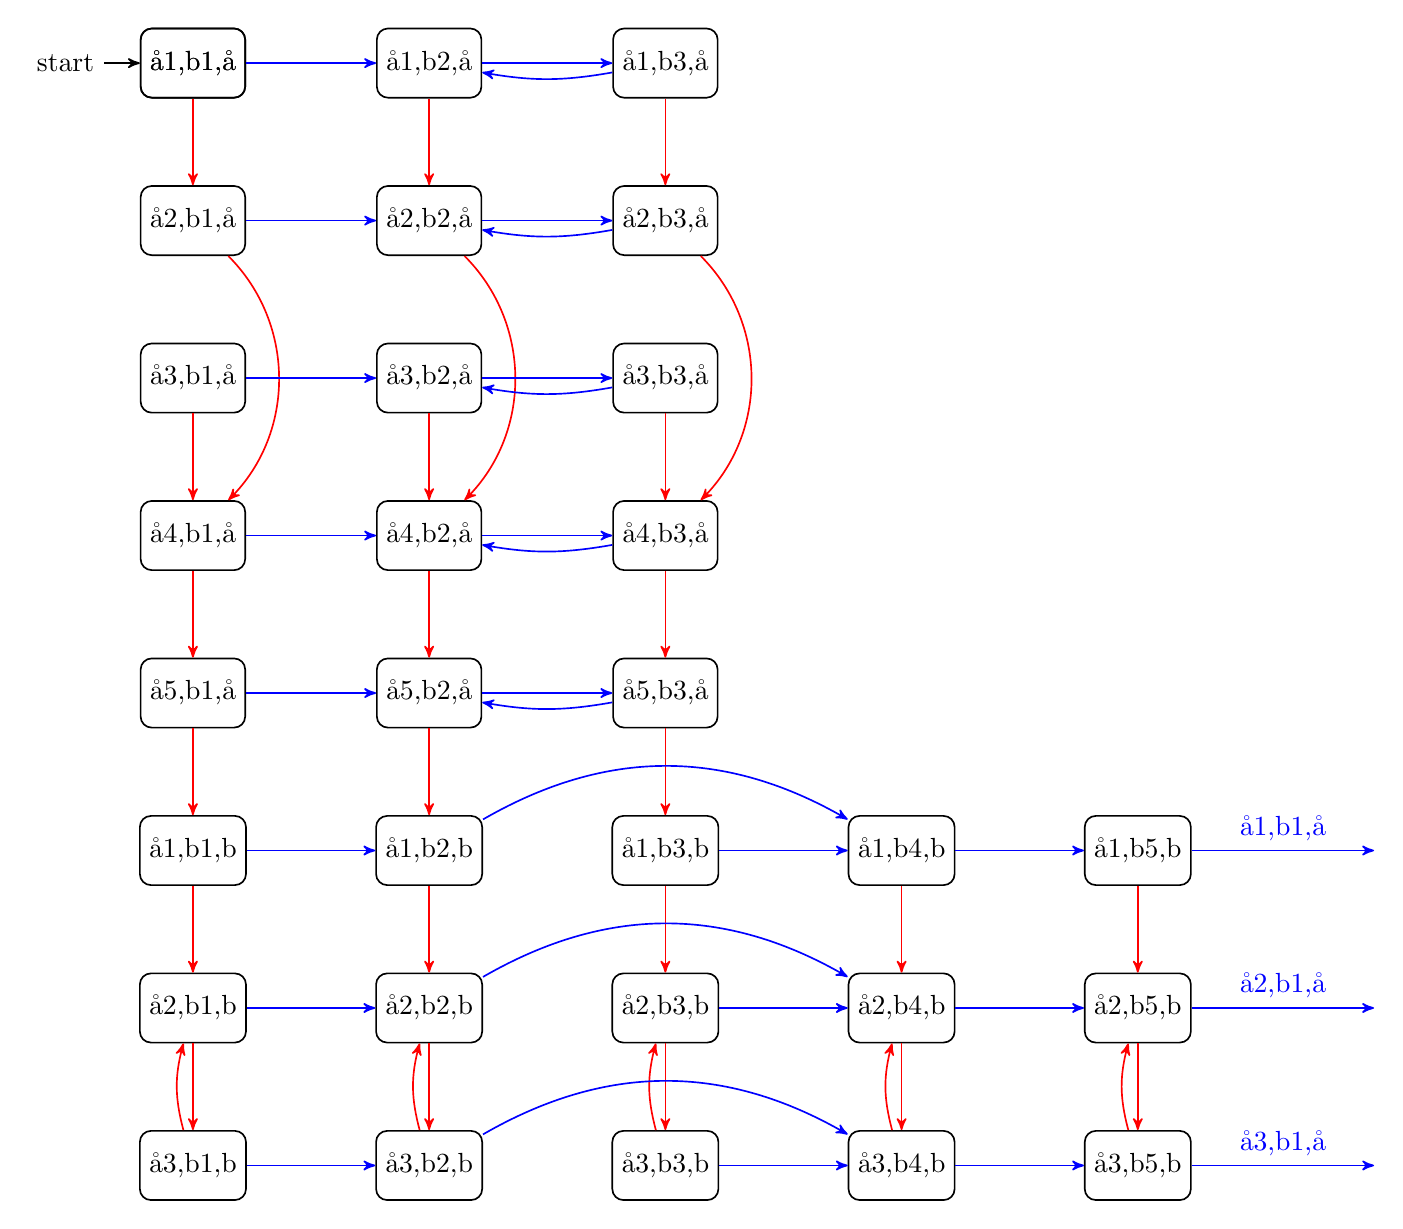
\begin{tikzpicture}[->,>=stealth',auto,node distance=2.8cm,semithick]
			\tikzset{every state/.append style={rectangle, rounded corners}}
			\node[state, initial] at (0,0) () {\r{a1},\g{b1},\r a};
			% 1: U
			% 2: while dran != a do
			% 3:	NOP
			% 4: K
			% 5: dran <- b

			% \foreach \y/\b in {0/b1,3/b2,6/b3} {
				% \foreach \x/\a in {0/a1,2/a2,4/a4,6/a5} {

			%! dran = a
			\foreach \b [count=\y from 0] in {b1,b2,b3} {
				\foreach \a [count=\x from 0] in {a1,a2,a3,a4,a5} {
					\node[state] at (\y*3,-\x*2) (\a_\b_a) {\r\a,\g\b,\r a};
				}
			}
			%! progress a
			\foreach \y in {b1,b2,b3} {
				\foreach \fromx/\tox in {a1/a2,a4/a5} {
					\draw (\fromx_\y_a) edge[red] (\tox_\y_a);
				}
				\draw (a2_\y_a) edge[red, bend left=45] (a4_\y_a);
				\draw (a3_\y_a) edge[red] (a4_\y_a);
			}
			%! progress b
			\foreach \x in {a1,a2,a3,a4,a5} {
				\foreach \fromy/\toy in {b1/b2,b2/b3} {
					\draw (\x_\fromy_a) edge[blue] (\x_\toy_a);
				}
				\draw (\x_b3_a) edge[blue,bend left=10] (\x_b2_a);
			}

			%! dran = b
			\foreach \b [count=\y from 0] in {b1,b2,b3,b4,b5} {
				\foreach \a [count=\x from 5] in {a1,a2,a3} {
					\node[state] at (\y*3,-\x*2) (\a_\b_b) {\r\a,\g\b,\g b};
				}
			}

			%! a5 => a1, dran <- b
			\foreach \y in {b1,b2,b3} {
				\draw (a5_\y_a) edge[red] (a1_\y_b);
			}

			%! progress a
			\foreach \y in {b1,b2,b3,b4,b5} {
				\foreach \fromx/\tox in {a1/a2,a2/a3} {
					\draw (\fromx_\y_b) edge[red] (\tox_\y_b);
				}
				\draw (a3_\y_b) edge[red,bend left=15] (a2_\y_b);
			}
			%! progress b
			\foreach \x in {a1,a2,a3} {
				\foreach \fromy/\toy in {b1/b2,b4/b5} {
					\draw (\x_\fromy_b) edge[blue] (\x_\toy_b);
				}
				\draw (\x_b2_b) edge[blue,bend left] (\x_b4_b);
				\draw (\x_b3_b) edge[blue] (\x_b4_b);
			}
			%! progress b, to a?_b1_a
			\foreach \a in {a1,a2,a3}
				\draw (\a_b5_b) edge[blue] node {\r\a,\g{b1},\r{a}} ++(3,0);
			% \draw (a2_b5_b) edge[blue] node {\r{a2},\g{b1},\r{a}} ++(3,0);
		\end{tikzpicture}
		\caption{Teilaufgabe a)}
	\end{figure}
\subsubsection*{b)}
Der Zustand $(a_2, b_2, b)$ gewährt durch den Zustand der geteilten Variable dem Prozess \texttt{b} den Zugang zum kritischen Abschnitt, während Prozess \texttt{a} in einer Warteschleife zwischen diesem und dem Zustand $(a_3, b_2, b)$ \textit{feststeckt}. Da Prozess \texttt{b} aufgrund schwacher Fairness irgendwann ausgeführt wird, verhindert diese Priorisierung Deadlocks. 

\AUFGABE{Der Algorithmus von Peterson}{}
\begin{enumerate}
\item Der Algorithmus führt eine zusätzliche globale Variable \texttt{letzter} ein, die festhält, welcher Prozess zuletzt den Eintritt in den kritischen Abschnitt gefordert hat. Der Prozess, der zuletzt gefordert hat, wartet nun, bis der andere Prozess seinen kritischen Abschnitt verlassen hat, signalisiert durch die globalen Variablen \texttt{adrin} und \texttt{bdrin}. Dadurch ist eindeutig geregelt, welcher der beiden Prozesse seinen kritischen Abschnitt betreten darf, falls beide fordern. 

Der Algorithmus hat mit dem Dekkers Algorithmus gemein, dass beide Prozesse eine Variable besitzen, die anzeigt, dass die ihren kritischen Abschnitt ausführen möchten. Im Gegensatz zu Dekkers Algorithmus, nimmt der Prozess, der nicht im kritischen Abschnitt ist, nicht seine Forderung zurück um einen Deadlock zu verhindern. Stattdessen wird die Reihenfolge vor dem betreten der Schleifen festgelegt, als die Reihenfolge mit der das Betreten gefordert wurde.
\end{enumerate}

\AUFGABE{CMPXCHG}{}
\begin{table}[h]
\centering
\begin{tabularx}{0.75\textwidth}{l | l}
\multicolumn{2}{c}{\texttt{common <- 0}}\\
\hline
\texttt{a} & \texttt{b}\\
\hline
\texttt{U} & \texttt{U} \\
\texttt{until common != 1 do} & \texttt{until common != 2 do} \\
\texttt{\hspace{2em}CMPXCHG(common, 0, 1)} & \texttt{\hspace{2em} CMPXCHG(common, 0, 2)} \\
\texttt{K} & \texttt{K} \\
\texttt{common <- 0} & \texttt{common <- 0}\\
\end{tabularx}
\caption{Thread-Safer Algorithmus mit CMPXCHG als atomare Anweisung}
\end{table}

\begin{table}[h]
\centering
\begin{tabularx}{0.75\textwidth}{l | l}
\multicolumn{2}{c}{\texttt{common <- 0}}\\
\hline
\texttt{a} & \texttt{b}\\
\hline
\texttt{until common != 1 do} & \texttt{until common != 2 do} \\
\texttt{\hspace{2em}CMPXCHG(common, 0, 1)} & \texttt{\hspace{2em} CMPXCHG(common, 0, 2)} \\
\texttt{common <- 0} & \texttt{common <- 0}\\
\end{tabularx}
\caption{Abgekürzter Thread-Safer Algorithmus mit CMPXCHG als atomare Anweisung}
\end{table}

\begin{figure}[htbp] 
  \centering
     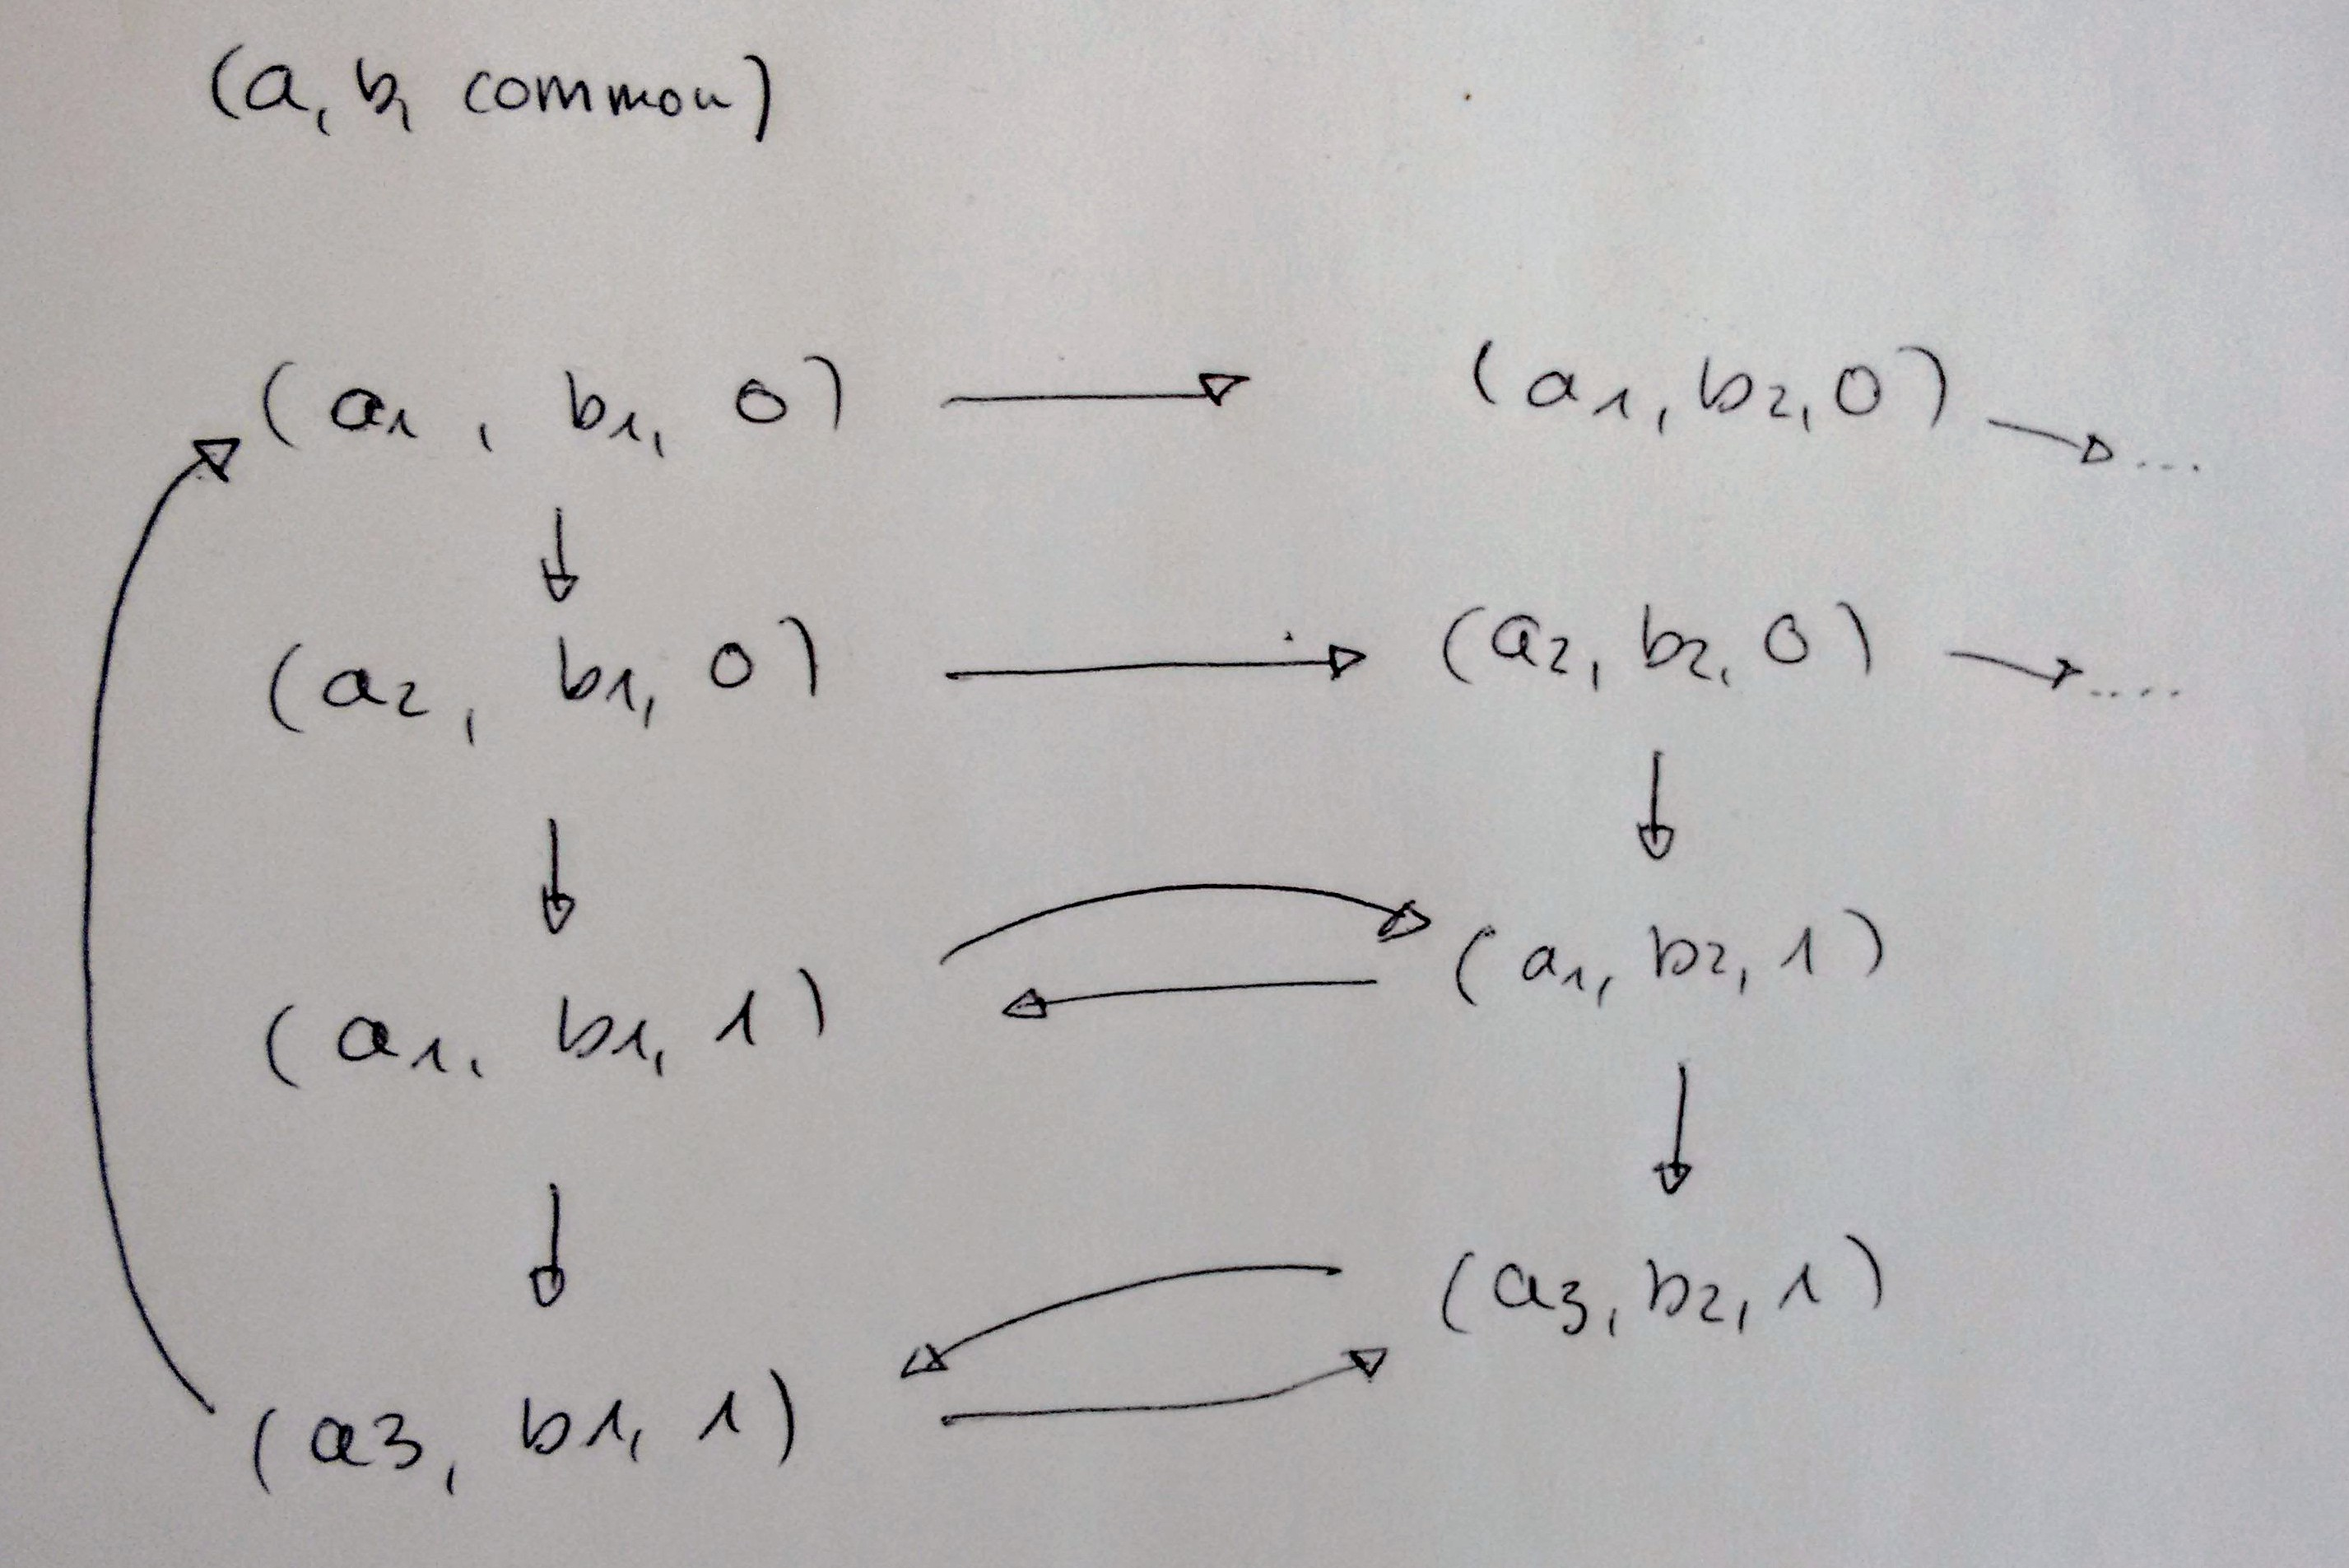
\includegraphics[width=0.8\textwidth]{zustand.jpg}
  \caption{Zustandsdiagramm des vereinfachten Algorithmus}
  \label{zsd}
\end{figure}

Aus dem in Abbildung \ref{zsd} dargestellten Zustandsdiagramm können wir die Korrektheit des Algorithmus nachvollziehen. Der Einfachheit halber ist in dem Diagramm nur der Fall dargestellt, in dem Prozess \texttt{a} den kritischen Bereich betritt. Der andere Fall ist symmetrisch.

Zunächst einmal lässt sich feststellen, dass nie der Zustand $(a_3, b_3, 1)$, $(a_3, b_3, 0)$ oder $(a_3, b_3, 2)$ angenommen wird. \textit{Mutual exclution} ist somit erfüllt.

Da die Variable \texttt{common} im kritischen Abschnitt zurück auf $0$ gesetzt wird und damit früher oder später (auf Grund schwacher Fairness) der Anfangszustand erreicht wird, wird irgendwann jeder Prozess die Möglichkeit haben, in seinen kritischen Abschnitt zu gelangen. Damit ist die \textit{Freedom from Starvation} sichergestellt.

Zu guter Letzt muss noch gezeigt werden, dass es keine Deadlocks gibt. Dies ist gewährleistet durch die \texttt{CMPXCHG} Funktion, welche in diesem Kontext nur das Überschreiben der geteilten Variable durch den Prozess, von dem sie zuerst aufgerufen wird, zulässt.

\end{description}
\end{document}
